\documentclass[12pt, a4paper]{article}

\usepackage{amsmath}
\usepackage{bm}
\usepackage{array}
\usepackage{amsmath}
\usepackage[portuguese]{babel}
\usepackage{chngpage}
\usepackage{float}
\usepackage[a4paper, margin=2cm]{geometry}
\usepackage{graphicx}
\usepackage{hyperref}
\usepackage{listings}
\usepackage{setspace}
\usepackage{tikz}
\usepackage{xcolor}

\usetikzlibrary{arrows, arrows.meta}

\lstdefinestyle{codestyle}{
    commentstyle=\color{teal},
    keywordstyle=\color{blue},
    numberstyle=\ttfamily\color{gray},
    stringstyle=\color{red},
    basicstyle=\ttfamily\footnotesize,
    breakatwhitespace=false,
    breaklines=false,
    keepspaces=true,
    numbers=none,
    showspaces=false,
    showstringspaces=false,
    showtabs=false,
    tabsize=4
}
\lstset{style=codestyle}

\title{\Huge \textbf{Computação Gráfica \\ \Large Trabalho Prático -- Fase III}}
\date{27 de abril de 2025}
\author{Grupo 3}

\begin{document}

\begin{center}
    
\includegraphics[width=0.25\textwidth]{res/cover/EE-C.eps}
\end{center}

\chardef\_=`_
\onehalfspacing
\setlength{\parskip}{\baselineskip}
\setlength{\parindent}{0pt}
\def\arraystretch{1.5}

{\let\newpage\relax\maketitle}
\maketitle
\thispagestyle{empty}

\vspace*{\fill}

\begin{adjustwidth}{-2cm}{-2cm} % These values only need to be large enough to center the table
    \begin{center}
        \begin{tabular}{>{\centering}p{0.25\textwidth}
                        >{\centering}p{0.25\textwidth}
                        >{\centering}p{0.25\textwidth}
                        >{\centering\arraybackslash}p{0.25\textwidth}}
            
\includegraphics[width=3.5cm]{res/cover/A104437.png} &
            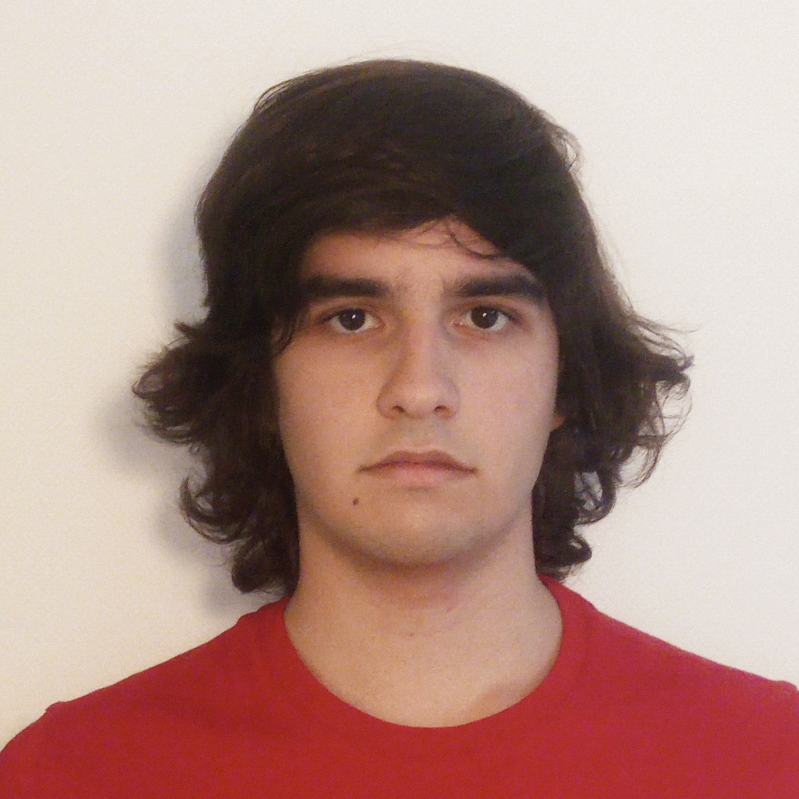
\includegraphics[width=3.5cm]{res/cover/A104348.png} &
            
\includegraphics[width=3.5cm]{res/cover/A90817.png} &
            
\includegraphics[width=3.5cm]{res/cover/A104179.png} \\

            Ana Oliveira & Humberto Gomes & Mariana Cristino & Sara Lopes \\
            A104437      & A104348        & A90817           & A104179
        \end{tabular}
    \end{center}
\end{adjustwidth}

\pagebreak

\begin{abstract}
    \noindent
    Nesta fase do trabalho prático, construiu-se sobre os programas \texttt{generator} e
    \texttt{engine} previamente desenvolvidos. No \texttt{generator}, a geração do Sistema Solar
    foi simplificada e modificada para suportar animação dos corpos celestes: rotações de velocidade
    constante e translações segundo curvas Catmull-Rom. Ademais, foi adicionada geração de modelos
    com base em \emph{patches} de Bézier. Na \texttt{engine}, foi adicionado suporte para a animação
    de objetos em cena e uma câmara em terceira pessoa. Na próxima fase, pretende-se desenvolver
    sobre o trabalho desta fase com a implementação de iluminação e aplicação de texturas aos
    objetos da cena.
\end{abstract}

\section{\emph{Generator}}

Nesta fase, o código do programa \texttt{generator} passou por um processo de limpeza, para o tornar
mais consistente, melhorar a sua legibilidade, e corrigir algumas falhas nas quais não se tinha
reparado em fases anteriores. Ademais, nesta fase, foi implementada a geração de modelos 3D com base
em \emph{patches} de Bézier.

\subsection{Alterações à Geração de Figuras Geométricas}

Em primeiro lugar, comece-se por mencionar o que não precisou de ser alterado. O \texttt{generator}
exporta os modelos 3D que gera no formato Wavefront OBJ \cite{wavefront-obj}, que foi descrito em
detalhe no relatório da primeira fase deste trabalho prático. Em suma, este formato consiste numa
sequência de vértices seguida de um conjunto de faces triangulares, e estas faces são definidas com
índices de vértices da sequência mencionada. Logo, já desde a primeira fase, a \texttt{engine} tira
proveito desta indexação no formato Wavefront OBJ para indexar os vértices dos modelos carregados
para a GPU, não tendo sido necessária qualquer alteração ao \texttt{generator} para gerar modelos
mais pequenos e que tiram proveito da \emph{cache} de vértices da GPU.

No entanto, é de notar que a geração de grelhas, presente em todas as figuras geradas, ainda podia
ser melhor otimizada para a \emph{cache} de vértices. Alguns métodos de indexação
\cite{optimal-grid} dão origem a modelos que são capazes de tirar um maior proveito da \emph{cache}
de vértices. No entanto, estes são mais complexos e envolvem a geração de triângulos degenerados,
pelo que se optou por não os utilizar, optando-se então por uma solução simples e fácil de
compreender (em \emph{scanline}).

Uma alteração ao processo de geração de modelos 3D foi a adição, a cada modelo, de um comentário que
enuncia os parâmetros utilizados na sua geração. Um exemplo de um destes comentários seria:

\begin{center}
\texttt{\# cone 1.000000 2.000000 4 2}
\end{center}

Ademais, o \emph{parser} de ficheiros Wavefront OBJ foi reimplementado com base em expressões
regulares, que o tornam mais eficiente e mais facilmente extensível. De momento, a única extensão
funcional em relação à fase anterior foi o suporte para comentários. No entanto, na próxima fase,
será necessário adicionar suporte para coordenadas de textura e vetores normais, e espera-se que o
uso de expressões regulares torne este processo mais fácil.

\subsection{Alterações à Geração do Sistema Solar}

A geração do Sistema Solar também sofreu alterações. Em primeiro lugar, para simplificar o seu
código, as posições dos corpos celestes já não são especificadas manualmente, mas sim geradas de um
modo pseudo-aleatório: no código apenas se especifica a distância de um corpo ao seu pai, $d$, um
ângulo $\theta \in \left [ 0, 2\pi \right [$ é gerado aleatoriamente, e a posição do corpo é
calculada da seguinte forma:

$$
x = d \cos \theta
\hspace{1cm}
z = d \sin \theta
$$

Ademais, a parametrização da geração do Sistema Solar também foi alterada. Agora, são pedidos ao
utilizador menos argumentos, que permitem um controlo semelhante da aparência da cena gerada:

\begin{center}
\small
\texttt{generator solarSystem [<sunScale> <rockyScale> <gasScale> <timeScale>] <directory>}
\end{center}

O utilizador agora pode, opcionalmente, definir a escala aplicada ao Sol (\texttt{sunScale}), aos
planetas rochosos e asteroides (\texttt{rockyScale}), e aos planetas gasosos (\texttt{gasScale}).
Ademais, nesta fase também foi adicionada animação à geração do Sistema Solar, que deu origem ao
parâmetro \texttt{timeScale}, que controla o quão rápidas as animações dos corpos celestes são. Num
caso extremo, é possível definir este parâmetro como zero para se obter uma cena estática.

Também se observa que o \texttt{generator} passa a criar uma diretoria com vários ficheiros, em vez
de apenas um ficheiro com a cena. Os novos ficheiros criados são os modelos de uma esfera, de um
\emph{torus}, e de um cometa, utilizados nos corpos celestes, nos seus anéis, e no cometa,
respetivamente. Isto é uma melhoria em relação à fase anterior, onde era esperado que o utilizador
gerasse estes modelos manualmente.

De seguida, foi descoberto um problema com a estrutura hierárquica do Sistema Solar a ser gerada
anteriormente. Os objetos eram agrupados em grupos conforme a sua atração gravítica: corpos a
orbitar o Sol eram colocados no grupo do Sol, e corpos a orbitar um planeta eram colocados no grupo
desse planeta. Logo, todos os corpos a orbitar um corpo $X$ estariam sujeitos a todas as
transformações de $X$, quando apenas se deseja que estejam sujeitos à sua translação: se o Sol
sofrer uma rotação, não se deseja que os planetas rodem o mesmo ângulo (estejam
\emph{tidally locked}). Para resolver este problema, caso um corpo celeste tenha outros corpos a
orbitá-lo, é colocado num grupo aninhado no qual são colocadas as suas transformações de escala e de
rotação. Como exemplo, segue-se a estrutura da Terra e da Lua:

\lstset{language=xml}
\begin{lstlisting}

<group>
    <transform>
        <translate ... />
    </transform>
    <group>
        <transform>
            <scale ... />
            <rotate ... />
        </transform>
        <models>
            <model file="sphere.3d" /> <!-- Terra -->
        </models>
    </group>
    <group>
        <transform>
            <translate ... />
            <scale ... />
            <rotate ... />
        </transform>
        <models>
            <model file="sphere.3d" /> <!-- Lua -->
        </models>
    </group>
</group>
\end{lstlisting}

Como se pode observar, no grupo exterior encontra-se a translação aplicada tanto à Terra como à Lua.
A Terra, como é orbitada pela Lua, é colocada num grupo interior com a sua escala e rotação. Quanto
à Lua, como nada a orbita, no seu grupo encontram-se as suas três transformações.

Também houve uma alteração à hierarquia de grupos das cinturas de asteroides. Anteriormente, cada
asteroide era um grupo, e todos estes grupos tinham o mesmo pai. Isto não era ideal para o
\emph{frustum culling}, porque era necessário verificar para todo o asteroide se ele se encontrava
ou não no \emph{view frustum}. Seria possível evitar vários testes se um grupo contivesse vários
asteroides e a esfera encapsuladora desse grupo não fosse visível.

Logo, para resolver este problema, cada cintura de asteroides é divida em subgrupos. Para determinar
o tamanho de cada subgrupo, procura-se que o comprimento do arco a que está associado seja o mesmo
que a largura da cintura de asteroides. Deste modo, a esfera que encapsula os asteroides não será
nem pequena nem grande demais, o que levaria a um maior número de testes de \emph{frustum culling}.
Assim, dados os raios externo ($R$) e interno ($r$) de uma cintura de asteroides, o seu número de
grupos pode ser calculado do seguinte modo:

$$
N = \left \lceil \frac{2 \pi \cdot \frac{R + r}{2}}{R - r} \right \rceil
  = \left \lceil \frac{\pi (R + r)}{R - r} \right \rceil
$$

Essencialmente, esta fórmula calcula quantas vezes a largura da cintura de asteroides ($R - r$) cabe
no perímetro da sua circunferência média. Com esta divisão, as esferas encapsuladoras dos grupos de
uma cintura de asteroides são visíveis na figura abaixo.

\begin{figure}[H]
    \centering
    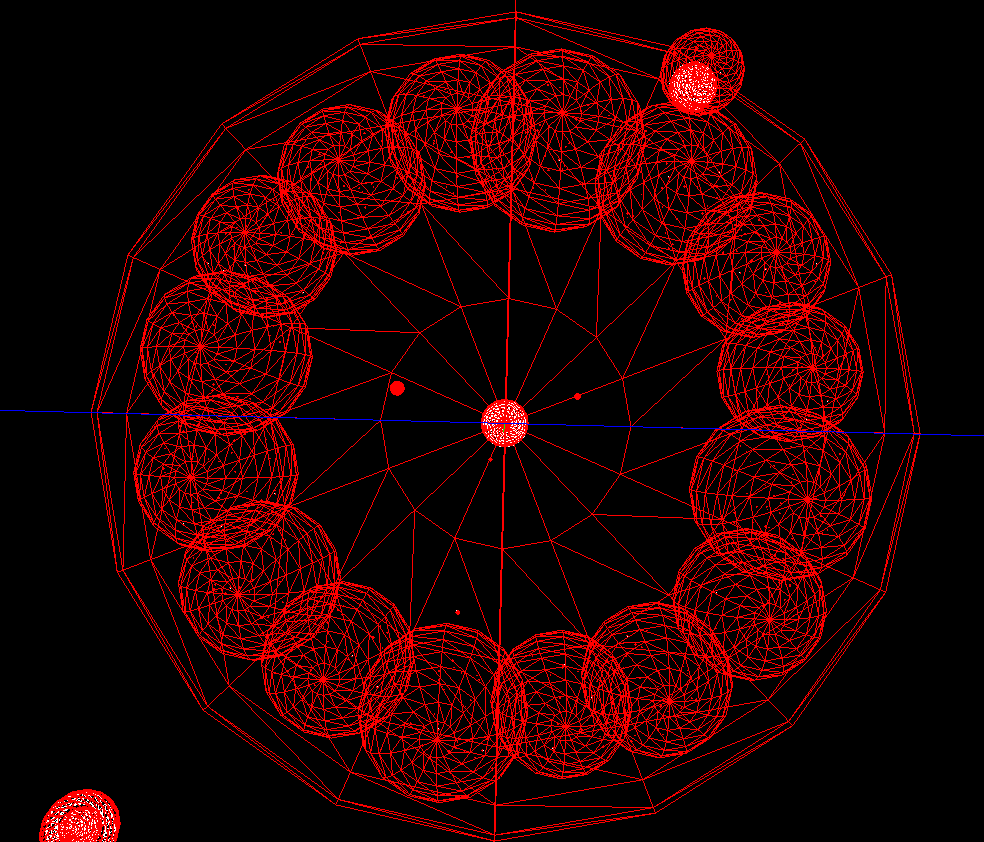
\includegraphics[width=0.5\textwidth]{res/phase3/AsteroidBeltBoundingSpheres.png}
    \caption{Esferas encapsuladoras dos grupos da cintura de asteroides interna.}
\end{figure}

Para adicionar animações ao Sistema Solar, as transformações \texttt{translate} e \texttt{rotate}
passam a ter um atributo \texttt{time}, que define a sua duração, ajustável pelo fator
\texttt{timeScale}, como explicado anteriormente. Ademais, para as translações, é necessário definir
os pontos de controlo de uma curva Catmull-Rom, que são uniformemente distribuídos por uma
circunferência:

$$
P_i = (r \cos \theta_{i}, \; y, \; r \sin \theta_{i}),
\hspace{1cm}
\theta_{i} = \frac{2 \pi i}{16}, \;
i \in \lbrace 0, 1, \ldots, 15 \rbrace
$$

Ademais, também se adicionou ao Sistema Solar um cometa, cujo modelo é gerado com base em
\emph{patches} de Bézier, e cujo movimento é ditado por uma curva Catmull-Rom (\texttt{translate}).

Por último, tal como foi feito com os modelos 3D, uma cena do Sistema Solar começa com um comentário
XML como o que pode ser visto abaixo, a enunciar os parâmetros com que foi gerada:

\begin{center}
    \texttt{<!-- solarSystem 1.000000 10.000000 10.000000 1.000000 -->}
\end{center}

\subsection{Geração de modelos com base em \emph{patches} de Bézier}

Foi adicionada ao \texttt{generator} a funcionalidade de gerar modelos 3D com base em \emph{patches}
de Bézier e um nível de tesselação, o que pode ser feito com a linha de comando abaixo:

\begin{center}
    \texttt{generator bezier <patchFile> <tessellation> <file>}
\end{center}

Após o \emph{parsing} do ficheiro de \emph{patches}, é necessário agregar o conjunto de pontos
associado a cada \emph{patch} com base nos seus índices
($p_{i j}, i, j \in \left \lbrace 1,2,3,4 \right \rbrace$). Depois, é necessário calcular as
coordenadas dos pontos no \emph{patch}. Matematicamente, é necessário considerar em primeiro lugar
as seguintes matrizes, notando que, nas expressões abaixo, $c$ corresponde a uma coordenada, $x$,
$y$ ou $z$:

$$
\def\arraystretch{1}
M =
\begin{bmatrix}
    -1 &  3 & -3 & 1 \\
     3 & -6 &  3 & 0 \\
    -3 &  3 &  0 & 0 \\
     1 &  0 &  0 & 0
\end{bmatrix}
\hspace{1cm}
P_c = \left [ {p_{i j}}_{c} \right ] _ {4 \times 4}
$$

Depois, os pontos na superfície de um \emph{patch} são dados por:

$$
\def\arraystretch{1}
p_c =
\begin{bmatrix}
    u^3 & u^2 & u & 1
\end{bmatrix}
M \, P_c \, M^T
\begin{bmatrix}
    v^3 \\ v^2 \\ v \\ 1
\end{bmatrix},
\hspace{1cm}
u, v \in \left [ 0, 1 \right ]
$$

Para gerar uma \emph{mesh} 3D, é necessário discretizar os valores de $u$ e de $v$. O intervalo
$\left [ 0, 1 \right ]$ pode ser dividido de acordo com o fator de tesselação, $T$:

$$
u_i = \frac{i}{T}
\hspace{1cm}
v_j = \frac{j}{T}
\hspace{1cm}
i, j \in \left \lbrace 0, 1, \ldots, T \right \rbrace
$$

Na prática, cada \emph{patch} é gerado iterando pelos valores possíveis de $u_i$ e de $v_j$,
calculando o valor de $p_c$ para as coordenadas $x$, $y$, e $z$. Em primeiro lugar, é incrementando
$v_j$ e só depois de $u_i$. Para a indexação destes vértices e para a geração das faces do
\emph{patch} é usado o mesmo método que foi utilizado para a geração do plano (método
\emph{scanline}, descrito em detalhe no relatório da primeira fase). Um detalhe de implementação é
que, para um melhor desempenho do \texttt{generator}, as matrizes da forma $M \, P_c \, M^T$ são
calculadas apenas uma vez por \emph{patch}.

\section{\emph{Engine}}

A \texttt{engine}, tal como o \texttt{generator}, para além de ter sido modificada para suportar as
funcionalidades apresentadas abaixo, sofreu uma rearquiteturação do seu código, para uma melhor
legibilidade e extensibilidade. Destas melhorias ao código, destaca-se o suporte para vários
\emph{shaders}, já em preparação para a 4ª fase do trabalho prático, a reimplementação da leitura de
\emph{input} do utilizador, agora baseada em eventos, e a simplificação da lógica de movimento das
câmaras, com a remoção de muito código duplicado utilizando conceitos de orientação aos objetos.

\subsection{Animação dos Objetos}

Um dos objetivos desta fase do trabalho é a implementação de animações, nomeadamente translações e
rotações dependentes da passagem do tempo, construindo sobre as transformações estáticas da fase
anterior. Mesmo assim, o projeto desenvolvido continua a suportar cenas com transformações
estáticas.

\subsubsection{Rotação}

A rotação dinâmica é muito semelhante à rotação estática, com a diferença de que o ângulo de rotação
passado à função \texttt{glm::rotate} é definido em função do tempo. Sendo $t$ o instante atual e
$T$ o período da animação (atributo \texttt{time} no ficheiro XML), tem-se:

$$
\theta_{t} = \frac{2 \pi t}{T}
$$

Opcionalmente, o atributo \texttt{clockwise="true"} pode ser definido no ficheiro XML, fazendo com
que a rotação ocorra no sentido dos ponteiros do relógio, ou seja, o ângulo usado para o cálculo da
matriz de rotação será o simétrico da expressão apresentada acima. Assim, com estes dois atributos,
uma rotação no ficheiro XML pode ser definida do seguinte modo, lembrado que o atributo
\texttt{clockise} é opcional:

\begin{center}
    \texttt{<rotate time="10"\ x="0"\ y="1"\ z="0"\ clockwise="true"\ />}
\end{center}

\subsubsection{Translação}

Para a implementação de translações animadas de objetos na cena, foram utilizada curvas de
Catmull-Rom. No ficheiro XML, é necessário especificar o período da animação e um conjunto de pelo
menos quatro pontos de controlo. Opcionalmente, um atributo \texttt{align} pode ser definido caso se
deseje rodar o objeto animado para acompanhar a curva:

\begin{lstlisting}

<translate time="50" align="true">
    <point x="0" y="0" z="0"/>
    ...
</translate>
\end{lstlisting}

Para obter a posição de um objeto animado num dado instante de tempo, é necessário, em primeiro
lugar, identificar o segmento da curva Catmull-Rom a interpolar e a posição temporal nesse segmento.
Para tal, é necessário antes normalizar o instante atual:

$$
\hat{t} = \frac{t N}{T},
$$

onde $N$ é o número de pontos de controlo. Depois, o segmento $s$ é dado pela parte inteira de
$\hat{t}$, e a parte fracionária de $\hat{t}$ é a posição desse segmento onde deve ser feita a
interpolação. Com o valor de $s$, podem determinar-se os pontos do segmento: $s$ será um índice na
lista de pontos de controlo, e desejam-se escolher os pontos $s - 1$, $s$, $s + 1$ e $s + 2$. Caso
um destes pontos esteja fora da lista, "dá-se a volta"{} à mesma e escolhe-se o ponto seguinte. Por
exemplo, caso se selecione o ponto $12$ numa lista de $10$ elementos, será escolhido o ponto de
índice $2$ ($s \mod N$).

Para calcular as coordenadas de um ponto, é preciso repetir o mesmo cálculo para $x$, $y$ e $z$. Por
exemplo, para a coordenada $x$ de um ponto, tem-se:

$$
\def\arraystretch{1}
P_x =
\begin{bmatrix} t^3 & t^2 & t & 1 \end{bmatrix}
\begin{bmatrix}
    -0.5 &  1.5 & -1.5 &  0.5 \\
       1 & -2.5 &    2 & -0.5 \\
    -0.5 &    0 &  0.5 &    0 \\
       0 &    1 &    0 &    0
\end{bmatrix}
\begin{bmatrix} {P_{s - 1}}_x \\ {P_{s}}_x \\ {P_{s + 1}}_x \\ {P_{s + 2}}_x \end{bmatrix}
$$

Repetindo este processo para as coordenadas $y$ e $z$, constrói-se um vetor que pode ser passado à
função \texttt{glm::translate} para a construção da matriz de translação. Depois, caso o atributo
\texttt{align} esteja definido, é necessário gerar uma matriz de rotação para que o objeto animado
acompanhe a curva. Para isso, é necessário, em primeiro lugar, calcular a derivada da curva:

$$
\def\arraystretch{1}
d_x =
\begin{bmatrix} 3 t^2 & 2 t & 1 & 0 \end{bmatrix}
\begin{bmatrix}
    -0.5 &  1.5 & -1.5 &  0.5 \\
       1 & -2.5 &    2 & -0.5 \\
    -0.5 &    0 &  0.5 &    0 \\
       0 &    1 &    0 &    0
\end{bmatrix}
\begin{bmatrix} {P_{s - 1}}_x \\ {P_{s}}_x \\ {P_{s + 1}}_x \\ {P_{s + 2}}_x \end{bmatrix}
$$

De um modo semelhante ao que foi feito com a posição, este cálculo é feito três vezes, uma vez para
cada coordenada, assim se obtendo um vetor $\vec{d}_n$. Depois, com base neste vetor, é possível
calcular os vetores em cada direção do objeto:

$$
\vec{r}_n = \vec{d}_n \times \vec{up}_{n - 1}
$$
$$
\vec{up}_n = \vec{r}_n \times \vec{d}_n
$$

Observando as expressões anteriores, repara-se que o vetor $\vec{up}$ deve ser armazenado de uma
iteração para a seguinte. A matriz de rotação, a ser aplicada depois da translação, é calculada do
seguinte modo, após normalizar os vetores apresentados:

$$
\def\arraystretch{1}
R = \begin{bmatrix}
                 &               &              & 0 \\
    \bf\hat{d}_n & \bf\hat{up}_n & \bf\hat{r}_n & 0 \\
                 &               &              & 0 \\
               0 &             0 &            0 & 1
\end{bmatrix}
$$

\subsection{\emph{Vertex Buffer Objects} (VBOs)}

Um dos objetivos do nosso grupo foi utilizar uma versão atual do OpenGL devido ao maior número de
funcionalidades suportadas e à possibilidade de depuração da \texttt{engine} com aplicações como
RenderDoc \cite{renderdoc}. A versão 4.6 do OpenGL foi escolhida, pelo que, já desde o começo da
primeira fase, o projeto desenvolvido utilizava não só VBOs, como também \emph{shaders},
obrigatórios no \emph{core profile} do OpenGL.

Em primeiro lugar, é importante conhecer como os \emph{shaders} de vértices e de fragmentos
desenvolvidos se encaixam na \emph{pipeline} de renderização. Considere-se o diagrama abaixo:

\begin{figure}[H]
    \centering
    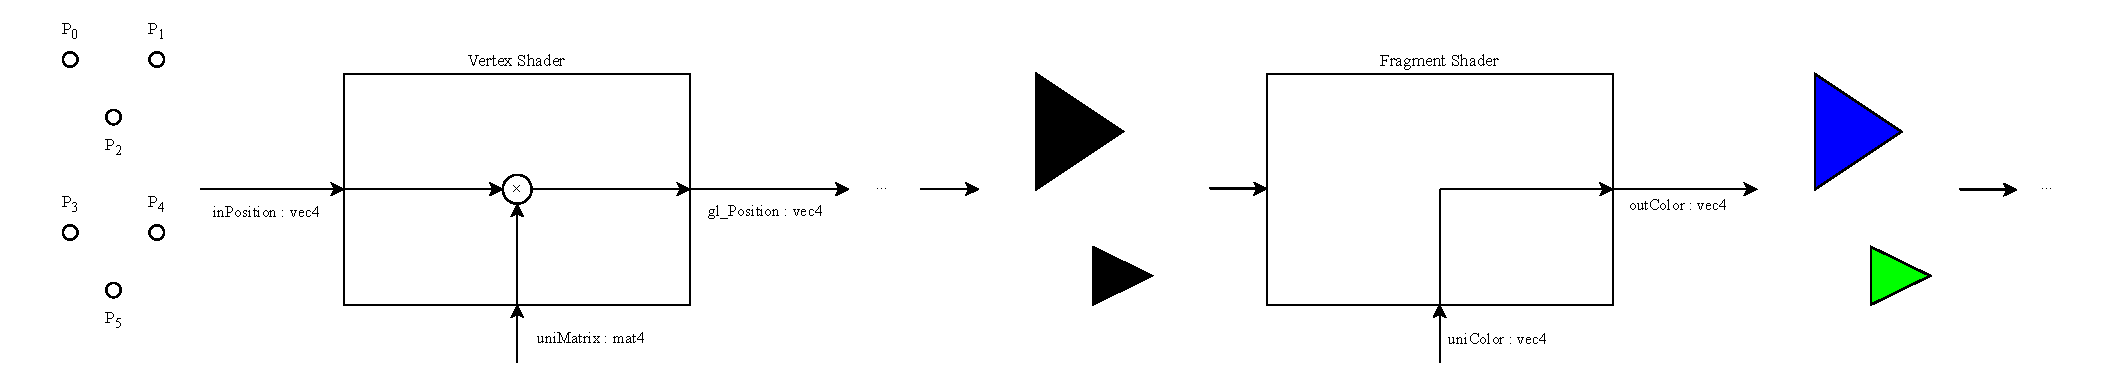
\includegraphics[width=\textwidth]{res/phase3/Shaders.pdf}
    \caption{Esquema dos \emph{shaders} desenvolvidos na \emph{pipeline} de renderização.}
\end{figure}

Como se pode observar, a única responsabilidade do \emph{shader} de vértices é multiplicar as
coordenadas das posições dos vértices que recebe por uma matriz de transformação passada numa
variável uniforme. Após o processamento dos vértices, dar-se-á o \emph{clipping}, a montagem das
primitivas, a divisão da perspetiva, a transformação pela \emph{viewport}, e a rasterização
\cite{vertex-post-processing}. Depois, para cada fragmento, o \emph{shader} de fragmentos será
invocado e, neste caso, atribuirá a todos os fragmentos das primitivas de um objeto a mesma cor,
passada como uma variável uniforme. Após a aplicação destes \emph{shaders} e algum processamento por
amostra, um objeto renderizado é colocado no \emph{framebuffer} para apresentação ao utilizador
\cite{per-sample-processing}. É de notar que a funcionalidade implementada por estes \emph{shaders}
é muito básica, apenas a necessária para o funcionamento correto da \texttt{engine} nesta terceira
fase do trabalho prático.

Após a criação dos \emph{shaders}, a \texttt{engine} carrega a cena e, para cada modelo, é criado um
\emph{Vertex Array Object} (VAO), algo que é obrigatório no \emph{core profile} do OpenGL. Com este
objeto vinculado, criam-se dois \emph{buffers}, um \texttt{GL\_ARRAY\_BUFFER}, no qual se armazenam
as posições dos vértices do modelo, e um \texttt{GL\_ELEMENT\_ARRAY\_BUFFER}, no qual se armazenam,
na forma de um \emph{array} de índices, a ordem em que estes vértices devem ser desenhados
\cite{glBufferData}. O uso de índices permite diminuir o tamanho dos modelos e tirar proveito da
cache de vértices da GPU. A figura abaixo mostra como estes três objetos estão relacionados:

\begin{figure}[H]
    \centering
    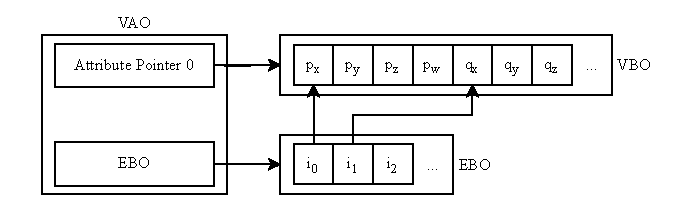
\includegraphics[width=\textwidth]{res/phase3/VAO.pdf}
    \caption{Organização do VAO, VBO, e EBO de um modelo.}
\end{figure}

Depois de criados estes objetos, para desenhar uma entidade na cena, basta vincular o seu VAO
correspondente e invocar a função \texttt{glDrawElements}.

O processo de envio de geometria para a GPU é semelhante para os eixos e para as representações
visuais das curvas de Catmull-Rom na cena. No entanto, não são criados \emph{arrays} de índices para
estes objetos, visto que não se espera que tenham vértices em duplicado. Então, a função usada para
desenhar estes objetos é \texttt{glDrawArrays}, e as primitivas são formadas com os vértices do VBO
pela ordem em que surgem no mesmo.

\subsection{Câmara em Terceira Pessoa}

Nesta fase, também foi implementada uma câmara em terceira pessoa, que  permite acompanhar um objeto
enquanto mantém uma perspetiva ligeiramente afastada, algo comum em diversos videojogos. Nesta
implementação, a câmara encontra-se constantemente orientada para o jogador, e acompanha os seus
movimentos a partir de uma posição relativa e ajustável.

Tal como a câmara orbital, a câmara em terceira pessoa utiliza coordenadas esféricas para definir a
sua posição em relação ao ponto de interesse, neste caso, o jogador. Esta posição é calculada com
base no raio $r$ (distância ao jogador), no ângulo azimutal $\phi$ (rotação horizontal), no
ângulo polar $\theta$ (inclinação vertical), e na posição do jogador ($P$). As coordenadas
cartesianas da posição da câmara são calculadas da seguinte forma:

$$x = P_x + r \sin \theta \cos \phi$$
$$y = P_y + r \cos \theta$$
$$z = P_z + r \sin \theta \sin \phi$$

Para garantir um comportamento estável da câmara, o raio é limitado de forma a que seja sempre
superior a $0$, evitando que a câmara se sobreponha ao jogador. O ângulo azimutal é mantido entre
$0$ e $2\pi$ por modularização, o que previne problemas de precisão de vírgula flutuante em rotações
prolongadas. O ângulo polar está restringido ao intervalo $[0.01, \pi - 0.01]$, para evitar os
problemas de inversão no vetor $\vec{up}$ da câmara que ocorrem fora deste intervalo.

Para movimentar o jogador, é necessário que tal seja feito na direção em que a câmara aponta,
$\vec{d} = \texttt{lookAt} - \texttt{position}$. No entanto, para o jogador não ``voar'', este vetor
é projetado no plano XZ:

$$
\vec{d'} = (d_x, 0, d_z)
$$

Para movimento lateral do jogador, é necessário calcular o vetor que o dirige. O vetor que aponta
para a direita do jogador é calculado do seguinte modo:

$$
\vec{r} = \vec{d'} \times \vec{up}
$$

Depois, ambos estes vetores são normalizados e utilizados para mover o jogador (diferentes vetores
são escolhidos conforme a tecla premida). A normalização destes vetores é importante para garantir
que garantir que a velocidade do jogador é constante.

Este modelo apresenta uma limitação: como $d$ é projetado no plano $XZ$, a câmara assume que o
jogador se move sobre terreno plano. Para jogos com terreno irregular e variação de elevação, este
comportamento deveria ser adaptado para ter em conta o mundo no movimento da câmara. Assim, seria
possível que o jogador se movesse na coordenada $y$, e também impedir que a câmara ficasse por baixo
do terreno.

O utilizador pode controlar a câmara de terceira pessoa utilizando as seguintes teclas:

\begin{itemize}
    \item \texttt{W/S}: Avançar ou recuar o jogador, respetivamente;
    \item \texttt{A/D}: Mover o jogador para a esquerda ou para a direita, respetivamente;
    \item Setas Cima / Baixo: Inclinar a câmara para cima ou para baixo, respetivamente;
    \item Setas Esquerda / Direita: Rodar a câmara à volta do jogador;
    \item \texttt{+/-}: Aproximar e afastar a câmara do jogador, respetivamente.
\end{itemize}

\section{Resultados Obtidos}

Nesta secção, procuram-se apresentar algumas capturas de ecrã da \texttt{engine} das novas cenas
criadas e das cenas fornecidas pela docência da UC.

\subsection{Novas Cenas e Cenas Modificadas}

Nesta fase, começaram-se por se desenvolver cenas simples, para se testarem as novas transformações
animadas:

\begin{figure}[H]
    \centering
    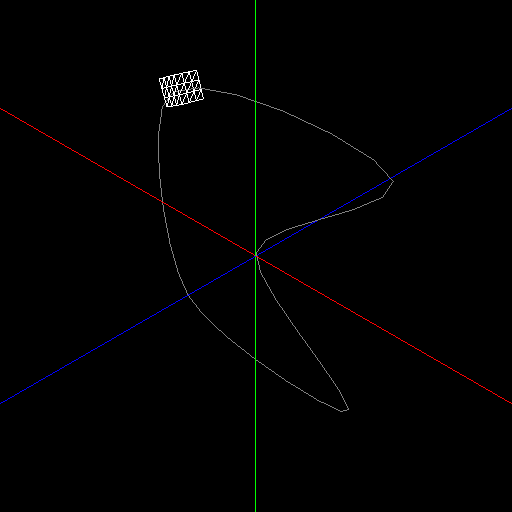
\includegraphics[width=0.30\textwidth]{res/phase3/results/Translation.png}
    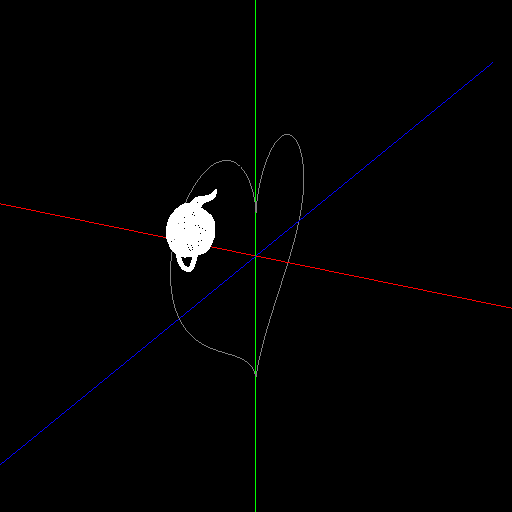
\includegraphics[width=0.30\textwidth]{res/phase3/results/TranslationHeart.png}
    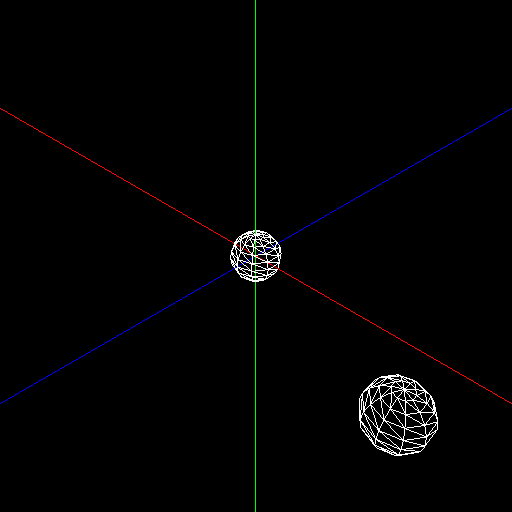
\includegraphics[width=0.30\textwidth]{res/phase3/results/Rotation.png}
    \caption{Novas cenas criadas nesta fase para teste das animações.}
\end{figure}

Depois, foram construídas cenas mais complexas, uma imitação do programa \texttt{glxgears} (com
rotação) e o Sistema Solar (gerado automaticamente), que podem ser vistas abaixo:

\begin{figure}[H]
    \centering
    
\includegraphics[height=0.30\textwidth]{res/phase3/results/glxgears.png}
    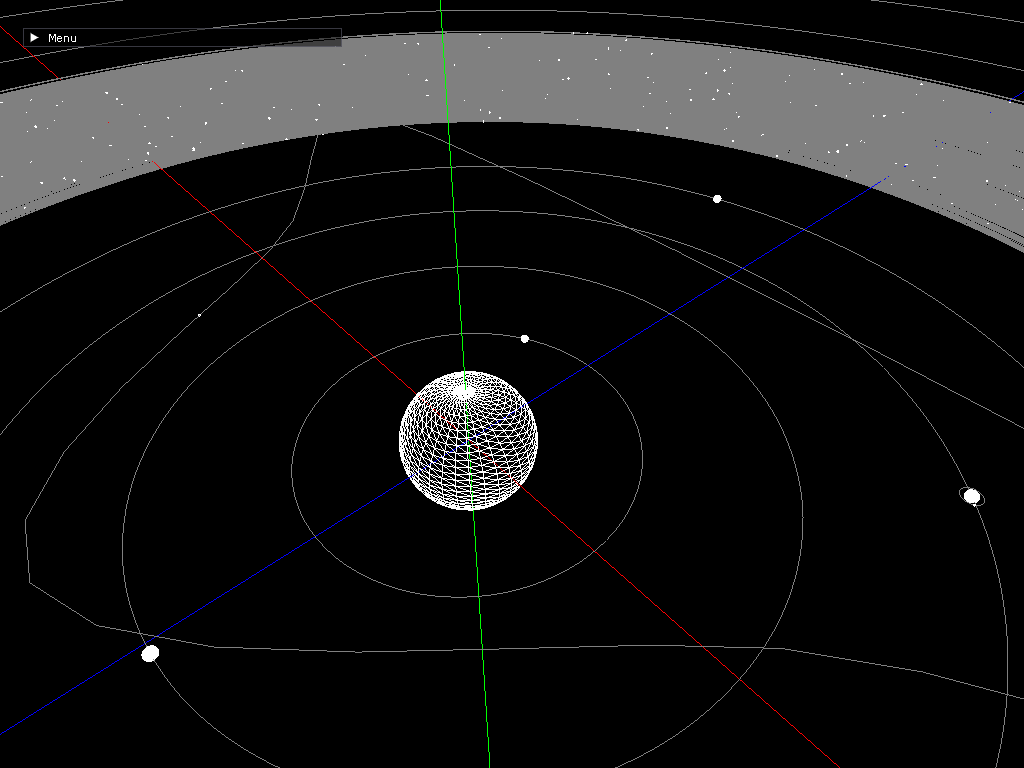
\includegraphics[height=0.30\textwidth]{res/phase3/results/SolarSystem.png}
    \caption{Novas cenas criadas nesta fase para teste das animações.}
\end{figure}

\subsection{Cenas Fornecidas pela Docência da UC}

A docência da UC forneceu, juntamente com o enunciado do trabalho, algumas cenas a serem testadas no
trabalho. A \texttt{engine} renderizou-as como esperado:

\begin{figure}[H]
    \centering
    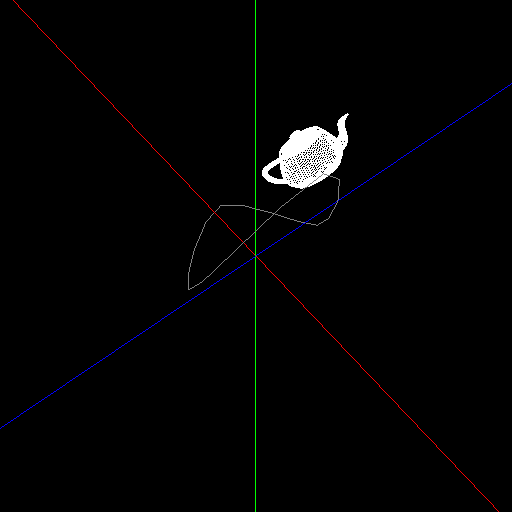
\includegraphics[width=0.4\textwidth]{res/phase3/results/Test1.png}
    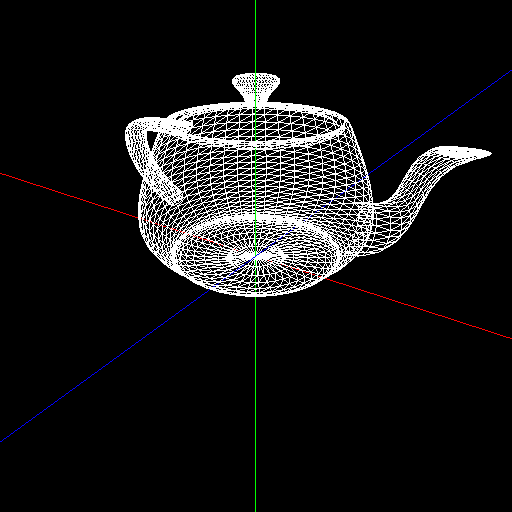
\includegraphics[width=0.4\textwidth]{res/phase3/results/Test2.png}
    \caption{Renderização das cenas de teste fornecidas pela docência da UC.}
\end{figure}

\section{Conclusão e Trabalho Futuro}

Consideramos que esta terceira fase deste trabalho prático foi concluída com sucesso. Em primeiro
lugar, não tivemos qualquer problema com a implementação das funcionalidades obrigatórias: as
animações e o uso de VBOs. No caso, já desde a primeira fase que o projeto utilizava VBOs para
armazenar os modelos 3D na memória da GPU. Além disso, foi implementada uma funcionalidade que tinha
sido um objetivo da fase anterior, a câmara em terceira pessoa. No entanto, não tivemos tempo para
implementar outras funcionalidades que tínhamos proposto na fase anterior: \emph{instanced
rendering} e \emph{object picking}. A implementação destas funcionalidades requiria algumas
melhorias à arquitetura da \texttt{engine}, como o suporte para vários \emph{shaders} previamente
mencionado. Foi possível fazer estas melhorias à \texttt{engine}, mas não sobrou tempo para
implementar as funcionalidades que tirariam proveito delas.

Para a próxima fase, desejamos implementar as funcionalidades obrigatórias pedidas, a iluminação e
aplicação de texturas aos objetos da cena, bem como tentar implementar as funcionalidades para as
quais não tivemos tempo nesta fase, \emph{instanced rendering} e \emph{object picking}.

\begingroup
\section{Bibliografia}
\renewcommand{\section}[2]{}

\begin{thebibliography}{9}
    \bibitem{wavefront-obj}
        ``Wavefront OBJ File Format Summary.'' FileFormat.Info. Accessed: Apr. 13, 2025. [Online.]
        Available: \url{https://www.fileformat.info/format/wavefrontobj/egff.htm}
    \bibitem{optimal-grid}
        ``Optimal Grid Rendering.'' Ignacio Castaño. Accessed: Apr. 14, 2025. [Online.] Available:
        \url{https://www.ludicon.com/castano/blog/2009/02/optimal-grid-rendering/}
    \bibitem{renderdoc}
        ``RenderDoc.'' RenderDoc Accessed: Apr. 14, 2025. [Online.] Available:
        \url{https://renderdoc.org/}
    \bibitem{vertex-post-processing}
        ``Vertex Post-Processing.'' OpenGL Wiki. Accessed: Apr. 13, 2025. [Online.] Available:
        \url{https://www.khronos.org/opengl/wiki/Vertex_Post-Processing}
    \bibitem{per-sample-processing}
        ``Per-Sample Processing.'' OpenGL Wiki. Accessed: Apr. 13, 2025. [Online.] Available:
        \url{https://www.khronos.org/opengl/wiki/Per-Sample_Processing}
    \bibitem{glBufferData}
        ``glBufferData.'' OpenGL 4.5 Reference Pages. Accessed: Apr. 15, 2025. [Online.] Available:
        \url{https://registry.khronos.org/OpenGL-Refpages/gl4/html/glBufferData.xhtml}
\end{thebibliography}
\endgroup

\end{document}
